\documentclass[a4paper,12pt]{report}
\usepackage[latin1]{inputenc}
\usepackage[T1]{fontenc}
\usepackage[english]{babel}
\usepackage{float}
\usepackage{hyperref}
\usepackage{listings}
\usepackage{cite}
\usepackage{acro}
\usepackage{graphicx}
\usepackage[nodayofweek]{datetime}

\DeclareGraphicsRule{*}{mps}{*}{}

% Commands
\newcommand{\HRule}{\rule{\linewidth}{0.5mm}} % Defines a new command for the horizontal lines

\begin{document}

	\begin{titlepage}
		\begin{centering}
		 
		%	HEADING SECTIONS
		
		\textsc{\textbf{\LARGE{Industrial Visit Report}}}\\[2cm]

		% \textbf{\textit{\large{A Project Report}}}\\[1.5cm]

		\large{submitted in partial fulfilment for the award of the degree of Bachelor of Technology in Computer Science and Engineering}\\[1.5cm]

		\large{by}\\[0.5cm]

		\textbf{Kevin Joseph     }\\
		{13400032 S7 R}\\[2cm]
		

		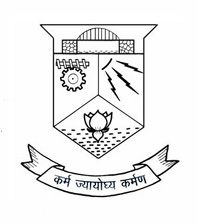
\includegraphics[width=5cm]{images/logo.jpg}

		\textsc{Department of Computer Science and Engineering}\\
		\textsc{College of Engineering Trivandrum}\\
		\textsc{Kerala}\\[0.5cm]
		\textsc{May 2017}\\
		\vfill % Fill the rest of the page with whitespace
		\end{centering}
	\end{titlepage}

	\begin{titlepage}
		\begin{centering}
			\textsc{\large{Department of Computer Science and Engineering}}\\
			\textsc{\large{College of Engineering Trivandrum}}\\[0.5cm]

			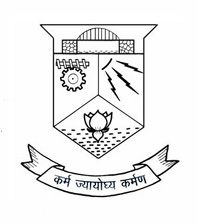
\includegraphics[width=5cm]{images/logo.jpg}\\[0.5cm]
			\textbf{\textit{\LARGE\textsc{{certificate}}}}\\[0.3cm]

		\end{centering}

		\begin{sloppypar}
		\large{This is to certify that this Industrial visit report is a bonafide record of the industrial visits undergone by Kevin Joseph (13400032), under our guidance towards partial fulfillment of the requirements for the award of Degree of bachelor of Technology in Computer Science and Engineering of the University of Kerala during the year 2016}\\[1.5cm]
		\end{sloppypar}

		\begin{minipage}{0.4\textwidth}
		\begin{flushleft}
		\begin{centering} \large
		\large{Mr. Sreelal S}\\
		\small{\textit{\textbf{Dept. of Computer Science and Engineering}}}\\[1.5cm]

		\end{centering}
		
		\end{flushleft}
		\end{minipage}
		~
		\begin{minipage}{0.5\textwidth}
		\begin{centering} \large
			\large{Mrs. Liji P I}\\
			\small{\textit{\textbf{Head of Department}}}\\
			\small{\textit{\textbf{Dept. of Computer Science and Engineering}}}\\
		\end{centering}
		\end{minipage}\\[1.0cm]

		\begin{flushleft}
		Place: Trivandrum\\
		Date:  11-05-2017\\
		\end{flushleft}
		\vfill % Fill the rest of the page with whitespace
	\end{titlepage}

	% TODO Ack before this
	\pagenumbering{roman}
	
	\newpage
	\tableofcontents
	\newpage

	\pagenumbering{arabic}
	\chapter*{\center{\textbf{\textsc{Sensomate Systems}}}}
	\addcontentsline{toc}{chapter}{Sensomate Systems}
	\newpage
		\section{About The Company}
		We visited Sensomate Systems on 21st January 2016. Sensomate Systems is a startup based in trivandrum with its office inside technopark (PHASE 1). We visited their office and were introduced to the work done by them and a overview of their products and software developement process. Sensomate is a company in the starup phase, but has had visible and continious growth in the previous years. They now have offices in Trivandrum, Chennai, Banglore, Canada and Saudi Arabia and clients across the world. The Company CEO is Krishnendu Gopalakrishnan and their team consists of 15 developers, 4 testers, 2 architects and 2 UX engineers.  
		\begin{figure}[H]
			\begin{centering}
				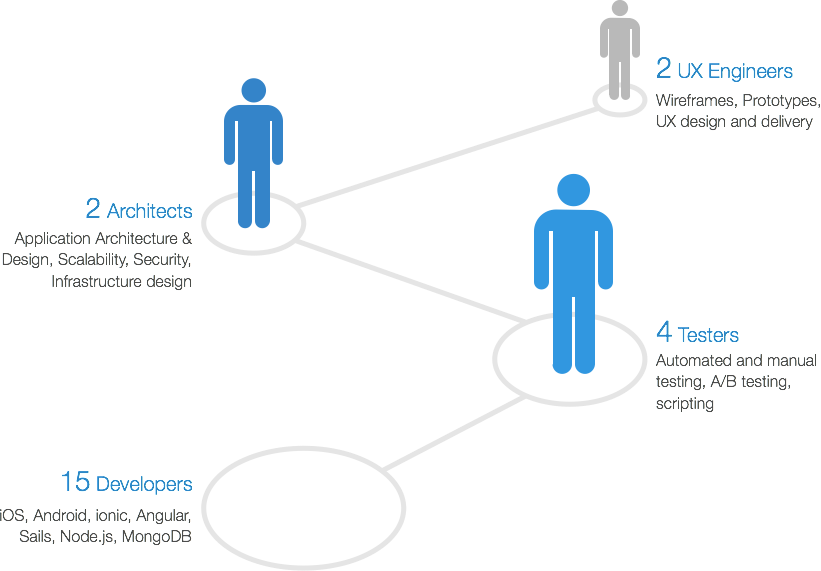
\includegraphics[width=10cm]{images/team.png}\\
				\caption{Sensomate Systems team.}
			\end{centering}
		\end{figure}
		Their mission is: ``Enchanting our customers, employees and shareholders by creating cutting edge and value add technology products and solutions that touches and leaves a lasting impression on how the world works and live.''
			\subsection{Technopark}
			Sensomate Systems is based in trivandrum, inside Technopark. Technopark is a technology park in Thiruvananthapuram, Kerala, India. It is the largest Information Technology park in Asia in terms of built up area. The park is dedicated to IT ventures. Launched in 1990, Technopark as of 2015 has 9.33 million square feet of built-up area, and is home to over 350 companies, employing nearly 60,000 professionals. Technopark is currently on an expansion mode by adding another 37 hectares as part of Phase III expansion and 423 acres as Technocity-an integrated IT township near Pallippuram. The policy of economic liberalisation initiated by the government of India in 1991 and the rapid growth of the global software industry during the 1990s substantially contributed to its growth. During the global financial crisis of 2007-2010, the park saw a period of reduced growth in 2009-10, where the exports recorded was only 2.8\% more than the previous year. As of 2017, Technopark accounts for about 70\% of IT exports from Kerala, which was 80\% in 2014.
			The units in Technopark include domestic firms, joint ventures and subsidiaries of foreign companies engaged in a wide variety of activities, which include embedded software development, smart card technology, enterprise resource planning (ERP), process control software design, engineering and computer-aided design software development, IT Enabled Services (ITES), process re-engineering, animation and e-business. Technopark is owned and administered by the Government of Kerala and is headed by a chief executive officer. In addition to this, it has a Governing Council and a Project Implementation Board, both of which include top officials of the government. Administrative offices, including that of the CEO, are housed in the Park Centre building. Technopark also hosts a Technology Business Incubation Cell under Kerala Startup Mission.
		\newpage
		\section{Products}
			\subsection{Proximity Beacons}
			Sensomate systems provides Bluetooth Low Energy(BLE) based proximity beacons separately and their also used in their other products like attendance system and schoolsafe.
			\subsection{Attendance System}
			The above mentioned proximity beacons can be used in an attendance and asset management system when clubbed with an interface and and bluetooth sensor devices. For the sensor side devices they used small android based devices to sense beacons and transmit data about them to a central server. The data on the central server is used to generate realtime statistics on an interface to be managed by a manager or group of managers.
			\subsection{Indoor Navigation System}
			Indoor navigation System is also based on the BLE beacons. Usually we use GPS for navigation, but a GPS on our smartphones can only give us an accuracy of upto 7-10m. This is not enough to navigate an indoor space, hence they used proximity beacons. The proximity beacons are used to mark places in an indoor space and the users' devices show position on an app. based on the beacons that they can sense. If the beacons are placed carefully, it is possible to attain a pretty good navigation system. The mention app is also developed by Sensomate as a part of this product.
			\subsection{SchoolSafe}
			This product was inspired by the problem of children missing stops or getting stuck, locked in school buses in Saudi Arabia. The solution was to have proximity beacons attatched to school id card and to track children in real time in buses and schools. This allows the system to send alerts to concerned people in case of unusual occurences and also provides a way to manage attendance. The main features include bus tracking, attendance management, parent teacher apps, context aware alerts etc.   
		\section{Software Development Lifecycle and Timeline}
			We were introduced to the software development process at Sensomate Systems. A modified version of the waterfall model was used. Each phase of development takes one or two weeks for normal application development.

			\begin{figure}[H]
				\begin{centering}
					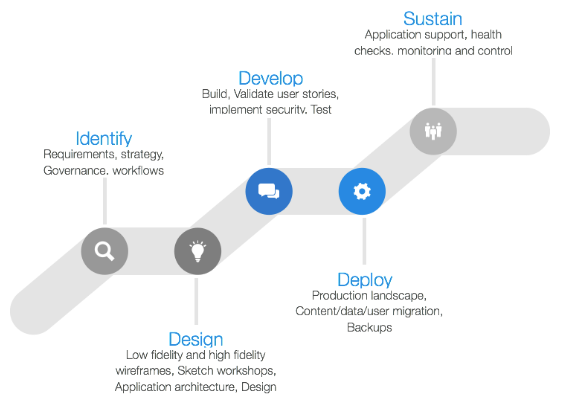
\includegraphics[width=10cm]{images/process.png}\\
					\caption{Software Development Process at Sensomate Systems.}
				\end{centering}
			\end{figure}

			\begin{figure}[H]
				\begin{centering}
					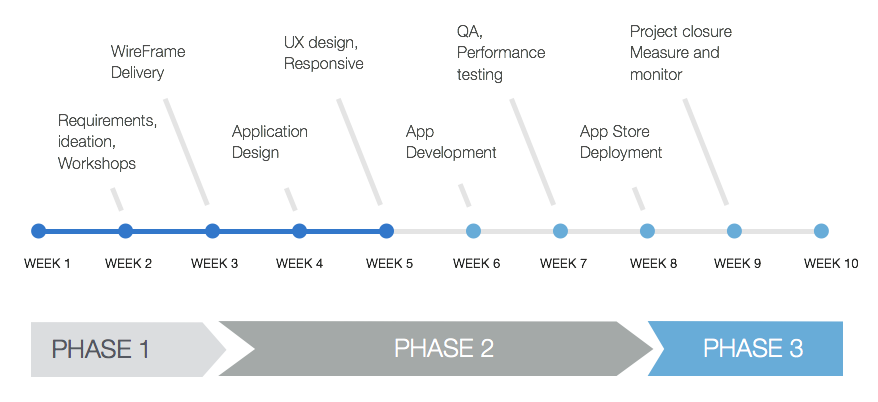
\includegraphics[width=10cm]{images/timeline.png}\\
					\caption{Software Development Timeline.}
				\end{centering}
			\end{figure}


			\subsection{Requirement, Ideation, Workshops}
				With spaced meetings and brainstorming sessions, a requirement specification document is prepared. The client confirms the specifications and any changes required, are done.
				Within two weeks time the requirements are finalized and any inconsistencies are worked out. 
			\subsection{Wireframe delivery}
				A wireframe of the app is designed using Balsamiq, or related tools, and the entire process of operation of the app is shown to the customer. A rough idea of the UI is also presented. The client goes through it and specifies any changes required, till a the wireframe design is consistent with the final expectation of the product.

			\subsection{Application design}
				The core funtionality of the app is analyzed and designed, the architecture, framework and language required are fixed. And the algorithms for each function of the app are designed. Testing each design unit seperately for correctness, a final design document is prepared.
			\subsection{Responsive UX Design}
				The final UX of the app is designed first. Material design guidelines are followed to ensure seamless operation within the app. The UX design is approved by the client before the functionalities are imbibed to it. Web apps require the extra hurdle of being responsive for operation from a mobile phone, this is ensured as well.
			\subsection{App development}
				The crux of the development process, the designs and algorithms fixed are coded within the required frameworks and attached to the UX to give correct, consistent functionality without compromise to performance. 
			\subsection{QA and Performance analysis}
				The app undergoes rigorous testing, where any bugs are found and fixed. The performance of the app is also considered and any lack in the same require rethinking of either the implementation or the design phase. 
			\subsection{Deployment}
				The app is deployed. Either as a website or to the relevant appstore. Hybrid apps are released to multiple appstores at the same time. The client ensures the availability of the app. Bug reporting facility is added for continued maintainance.
			\subsection{Maintainance}
				The project is wound up and any documentation updates are done. Any changes or updations needed are ensured through continued maintainance of the system.

		\section{Topics Discussed}
			\subsection{Data Analytics}
			Data analysis, also known as analysis of data or data analytics, is a process of inspecting, cleansing, transforming, and modeling data with the goal of discovering useful information, suggesting conclusions, and supporting decision-making. Data analysis has multiple facets and approaches, encompassing diverse techniques under a variety of names, in different business, science, and social science domains.

			Data analytics is a key area of focus for sensomate. All the major products of Sensomate Systems relies on Data analytics. The realtime attendance system Schoolsafe is the perfect example. It collects information about students in school and bus premises and stores and analyzes the data to take various decisions and display them to end users. The row data for this is the present/absent value for each student in regular intervals of time under each sensor. This data is stored in a centralized database and processed. The processing and querying is done by Influxdb, a time series database. The processed data can be used to determine whether a particular student was present in an area at a given time.
			\subsection{Realtime Web}
			The real-time web is a network web using technologies and practices that enable users to receive information as soon as it is published by its authors, rather than requiring that they or their software check a source periodically for updates. This is a major transition from old style websites where user just go to a website and refreshes the page everytime they want to get new updates. Realtime web is a huge area of development for Sensomate Systems. It is a vast area where a lot of new things happen everyday.

			The evolution of Javascript as a full stack development language accelerated the growth of realtime web. Realtime websites started to become a trend with the introduction of Ajax by Google. Ajax is a javascript library which can communicate with server side without refreshing the page. Jquery was also introduced as a easy-to-use and powerful library for javascript to attract a lot of companies in this area and it is still one of the most used javascript frameworks. The introducion of Node.js and AngularJs was a major milestone in Realtime web history. It was evolved into MEAN stack (Mongo Express Angular Node) and its the current choice of framework for most companies.

			In Sensomate, All realtime websites are developed using MEAN stack. The same can be developed as a mobile application using IONIC framework.
			\subsection{Mobile Application}
			With the steady growth in smartphone users worldwide, Mobile Application development has became a key area of focus in the last decade among many companies. In Sensomate systems all applications are developed in a framework called Ionic. The advantage of this library is that it is cross platform. Once the coding phase is done, we can compile it to any platform (Android, IOS, Firefox OS, Web etc) with just a few clicks. Since Ionic is based on AngularJS, it takes much lesser time than developing native apps. Also more libraries, themes and designs are available online for Ionic Framework. Use of a Ionic also ensures that the application will be consistant among any mobile phones/ tablets. We can ensure this by using a responsive design.
			However, Since Ionic is a web based framework, it has a slight performance impact and it is easily noticable in low end phones. But since all smartphones nowadays have lots of processor speed and memory, this wouldn't be a problem.
			\subsection{Internet of Things}
			The Internet of things (IoT) is the inter-networking of physical devices, vehicles (also referred to as "connected devices" and "smart devices"), buildings, and other items embedded with electronics, software, sensors, actuators, and network connectivity which enable these objects to collect and exchange data.In 2013 the Global Standards Initiative on Internet of Things (IoT-GSI) defined the IoT as "a global infrastructure for the information society, enabling advanced services by interconnecting (physical and virtual) things based on existing and evolving interoperable information and communication technologies" and for these purposes a "thing" is "an object of the physical world (physical things) or the information world (virtual things), which is capable of being identified and integrated into communication networks". The IoT allows objects to be sensed or controlled remotely across existing network infrastructure, creating opportunities for more direct integration of the physical world into computer-based systems, and resulting in improved efficiency, accuracy and economic benefit in addition to reduced human intervention. When IoT is augmented with sensors and actuators, the technology becomes an instance of the more general class of cyber-physical systems, which also encompasses technologies such as smart grids, virtual power plants, smart homes, intelligent transportation and smart cities. Each thing is uniquely identifiable through its embedded computing system but is able to interoperate within the existing Internet infrastructure. Experts estimate that the IoT will consist of about 30 billion objects by 2020.
			All the products developed by Sensomate are examples of IOT products. This indicates that Sensomate Systems is an innovative company which follows latest trend in technology, and keeps updated.
			\subsection{Content Managemant Systems}
			Content management, is a set of processes and technologies that supports the collection, managing, and publishing of information in any form or medium. When stored and accessed via computers, this information may be more specifically referred to as digital content, or simply as content. Digital content may take the form of text, multimedia files, or any other file type that follows a content lifecycle requiring management. Wordpress is one of the most famous Content Management system, which is used to host a blog and manage it.
			Along with developing IOT Applications and integrating Data Analytics, It is crucial that we need to present the information obtained to the end users. Also the users should be able to view/edit or manage the data they want to. Else the information obtained is useless. For this, Content management systems are developed. In the product Schoolsafe, The Online Dashboard (Used by parents, teachers, staffs, managers) and the Mobile application are examples of CMS. They allow users to manage the students, attendance etc.
	
\end{document}